\subsection{Pareto fronts}
\label{sec:pareto}

\begin{figure} 
  \centering
  \begin{subfigure}[b]{0.45\linewidth}
    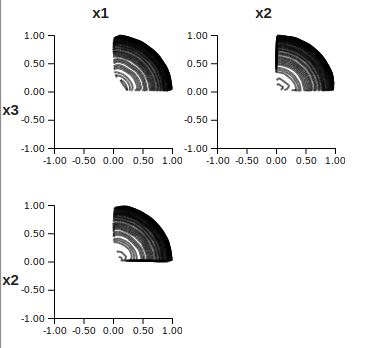
\includegraphics[width=\textwidth]{hsp_3d_pareto.png}
    \caption{3D}
    \label{fig:pareto:3d} 
  \end{subfigure} 
  ~
  \begin{subfigure}[b]{0.45\linewidth}
    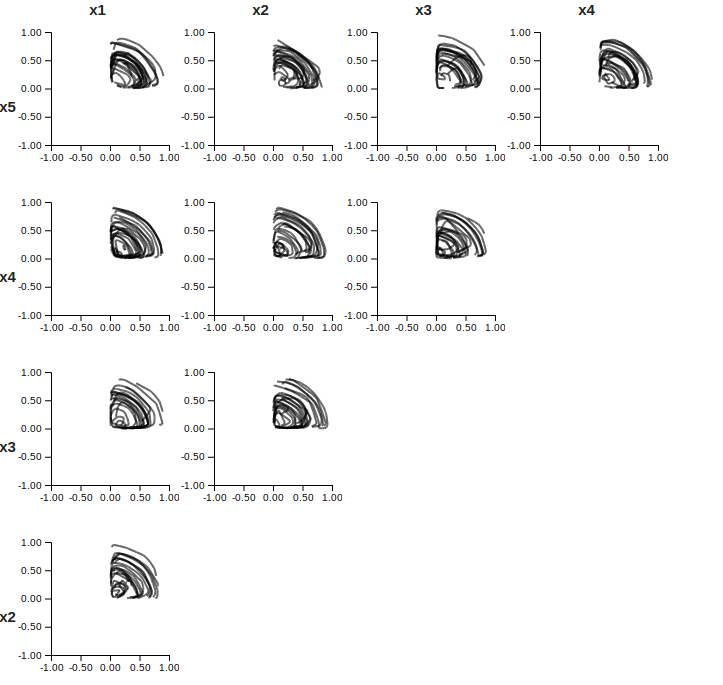
\includegraphics[width=\textwidth]{hsp_5d_pareto.png}
    \caption{5D}
    \label{fig:pareto:5d} 
  \end{subfigure}
  \caption[Hypersliceplorer views of spherical Pareto fronts in 3D and 5D.]{%
    Hypersliceplorer views of spherical Pareto fronts in 3D 
    (\subref{fig:pareto:3d}) and 5D (\subref{fig:pareto:5d}). 
    The smoothest possible Pareto front is the positive orthant of a 
    hypersphere.  From
    the Hypersliceplorer view we can clearly see the concentric arcs. Each
    arc allows the user to compare the trade-offs between two objectives 
    given that all other objectives are fixed. Changing from one arc to 
    another means changing other objective settings.
  }
  \label{fig:paretoex}
\end{figure}

%We can also use Hypersliceplorer to visualize the Pareto front used to
%understand trade-offs in multi-objective optimization. 
A Pareto front (also
known as the efficient frontier) is the set of all points that are optimal with
respect to some trade-off between objectives. Algorithms such as the skyline
algorithm~\cite{Borzsony:2001} or NSGA-II~\cite{Deb:2002} can extract these
points automatically. The issue with multi-objective optimization is this
trade-off is not always known. Thus visual analysis of the trade-offs is
necessary. With two objectives, this can be visualized using a scatterplot or
line plot of the two objectives against each other. 

In more than two dimensions this is no longer a curve, it is a hull. The common
technique is to use a scatterplot matrix with discretely sampled points. This, however, hides the trade-offs between
points in the other dimensions. Instead, we can examine the hull of the 
Pareto front by slicing using Hypersliceplorer.

The smoothest possible Pareto front is a sphere in the positive orthant of the objective
space. In order to illustrate our technique we show a 3D and 5D
positive orthant section of a sphere in \autoref{fig:paretoex}.  Each arc is
the trade-off holding all other parameters fixed.  In the multi-dimensional
view, setting the focus point is analogous to fixing all but two parameters.
Thus, in one plot one can directly see the trade-off between two of the 
objective measures given that all other objectives are held in place. However,
the user can also see at a glance what are the \emph{possible} trade-off curves
for a pair of objectives. This helps the user to understand what are the costs
and benefits of changing one of the remaining objectives.

\begin{figure} 
  \centering
  \begin{subfigure}[b]{0.45\linewidth}
    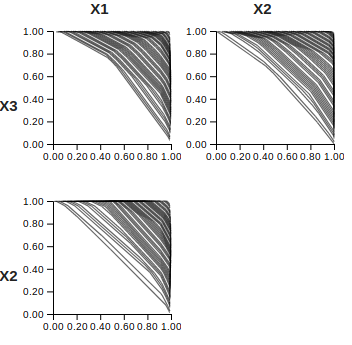
\includegraphics[width=\textwidth]{hsp_dltz1_3.png}
    \caption{3-objective}
    \label{fig:dltz:3}
  \end{subfigure}
  ~
  \begin{subfigure}[b]{0.45\linewidth}
    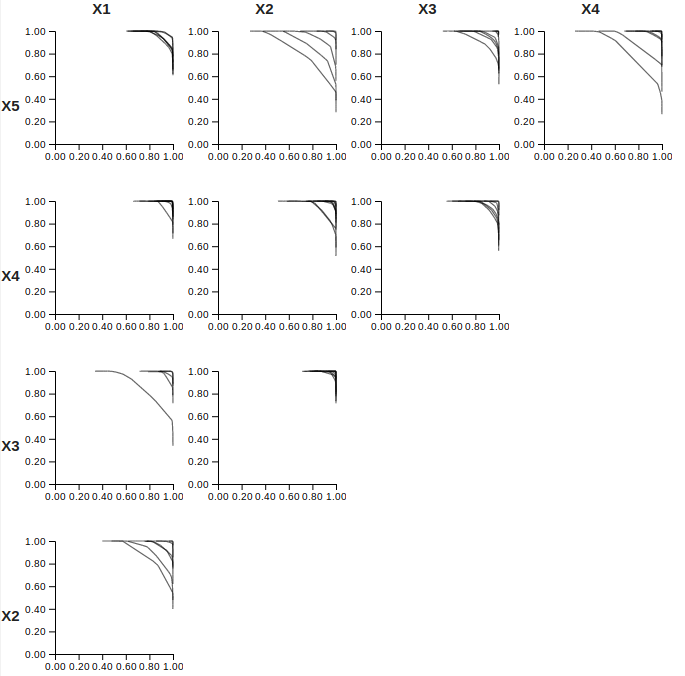
\includegraphics[width=\textwidth]{hsp_dltz1_5.png}
    \caption{5-objective}
    \label{fig:dltz:5}
  \end{subfigure}
  \caption[Visualization of the 3-objective and 5-objective DLTZ1 problems in Hypersliceplorer.]{%
    Visualization of the 3-objective~(\subref{fig:dltz:3}) and 
    5-objective~(\subref{fig:dltz:5}) DLTZ1 problems~\cite{Deb:2002a} in
    Hypersliceplorer. The DLTZ1 Pareto front is a hyperplane that cuts 
    diagonally across the objective dimensions. In the 3-objective case we 
    can see the slices of the hyperplane. The NSGA-II~\cite{Deb:2002} 
    algorithm tends to push points towards one objective. This becomes much
    more pronounced in higher dimensions (\subref{fig:dltz:5}) where the
    Pareto front is squared off.
  }
  \label{fig:dltz} 
\end{figure}

I also show a popular multi-objective test problem, DLTZ1~\cite{Deb:2002a}
with 5 objectives.  I find the Pareto points using the NSGA-II~\cite{Deb:2002}
algorithm.  I used the same settings for the algorithm as in Deb et 
al.~\cite{Deb:2002a}. In real-world situations, the Pareto front is not
convex. One can use, for example, alpha shapes~\cite{Edelsbrunner:1983} to
generate a non-convex hull of a set of points. For this example, we use the
convex hull of the points generated using the quickhull~\cite{Barber:1996}
algorithm since the Pareto front of DLTZ1 is convex.  The Pareto front is a
hyperplane that cuts diagonally across the objective dimensions. In the
3-objective case (\autoref{fig:dltz:3}) we can see how the NSGA-II algorithm is 
getting close to fitting the points to the hyperplane. It does not find it
exactly though which is why the lines appear bent in the figure. In addition,
NSGA-II pushes some points out to the maximum value for each objective.
This creates the horizontal and vertical lines at the edges of the plots.
This becomes much more pronounced in higher dimensions (\autoref{fig:dltz:5})
where the Pareto front appears as a corner shape.

